\documentclass{simple}

\title[Cum să fii bun la sex]{Cum să fii bun la sex}
\institute{Excursie, Moieciu}
\author[Familia D]{Familia D \\
    fam.d@sexrox.xxx}
\date{15 martie 2025}

\begin{document}

\frame{\titlepage}

\begin{frame}{Never don't give up!}
  \pause
  \begin{figure}
    \centering
    
\includegraphics[width=0.7\textwidth]{img/best-anal-sex-scene.jpg}
  \end{figure}
\end{frame}

\begin{frame}{Aveți grijă de nevoile primare!}
  \pause
  \begin{figure}
    \centering
    
\includegraphics[width=0.55\textwidth]{img/eating-porn-scene.jpg}
  \end{figure}
\end{frame}

\begin{frame}{Nu fiți autiști! Read the room!}
  \pause
  \begin{figure}
    \centering
    
\includegraphics[width=0.7\textwidth]{img/porn-director.png}
  \end{figure}
\end{frame}

\begin{frame}{Nu fiți egoiști și autiști!}
  \pause
  \begin{figure}
    \centering
    
\includegraphics[width=0.4\textwidth]{img/feedback-porn-without-link.jpg}
  \end{figure}
\end{frame}

\begin{frame}{}
  \centering
  \LARGE
  Analiză sondaj
\end{frame}

\begin{frame}{}
  \centering
  \LARGE
  De ce este sexul important?
\end{frame}

\begin{frame}{Rolurile sexului}
  \centering
  \Large
  \pause
  reproducere \\
  \vspace{1cm}
  \pause
  recreere \\
  \vspace{1cm}
  \pause
  romantism
\end{frame}

\begin{frame}{Cel mai mare organ sexual al corpului?}
  \centering
  \LARGE
  \pause
  creierul
\end{frame}

\begin{frame}{Senzualitate și emoție}
  \centering
  \pause
  \vspace{5mm}
  \textit{Sex without love is merely healthy exercise.} \\
  \vspace{3mm}
  \hfill \textit{Robert A. Heinlein} \\
  \pause
  \vspace{1cm}
  \textit{Sex without love is as hollow and ridiculous as love without sex.} \\
  \vspace{3mm}
  \hfill \textit{Hunter S. Thompson}
\end{frame}

\begin{frame}{Fizică / biologică și psihologică / emoțională}
  \centering
  \LARGE
  \pause
  prezență \\
  \vspace{1cm}
  \pause
  conexiune \\
  \vspace{1cm}
  \pause
  contact \\
  \vspace{1cm}
  \pause
  comunicare
\end{frame}

\begin{frame}{Ce înseamnă să fii bun la ceva?}
  \centering
  \Large
  \pause
  bun la capacitatea ta \\
  \vspace{1cm}
  \pause
  de evitat (dar nu exclus) comparațiile \\
  \vspace{1cm}
  \pause
  proces, nu finalitate
\end{frame}

\begin{frame}{Cum ajungi să fii bun la ceva?}
  \centering
  \Large
  \pause
  îți place \\
  \vspace{1cm}
  \pause
  te antrenezi \\
  \vspace{1cm}
  \pause
  ești acolo, ești prezent (nu doar fizic) \\
  \vspace{1cm}
  \pause
  ești autentic (true), nu te minți, nu ești mimetic
\end{frame}

\begin{frame}{Cum ajungi să fii bun la sex?}
  \centering
  \Large
  \pause
  îți place \\
  \vspace{1cm}
  \pause
  te antrenezi \\
  \vspace{1cm}
  \pause
  ești acolo, ești prezent (nu doar fizic) \\
  \vspace{1cm}
  \pause
  ești autentic (true), nu te minți, nu ești mimetic
\end{frame}

\begin{frame}{Cum ajungi să nu fii bun la sex?}
  \centering
  \Large
  \pause
  nu îți place \\
  \vspace{1cm}
  \pause
  nu te antrenezi \\
  \vspace{1cm}
  \pause
  nu ești acolo, nu ești prezent \\
  \vspace{1cm}
  \pause
  nu ești autentic, te minți, ești mimetic, joci la impresie
\end{frame}

\begin{frame}{De ce nu îți place sexul?}
  \centering
  \Large
  \pause
  probleme fizice / biologice \\
  \vspace{1cm}
  \pause
  blocaje psihologice / emoționale (you problem) \\
  \vspace{1cm}
  \pause
  persoana nepotrivită (him / her problem) \\
  \vspace{1cm}
  \pause
  părerea ta despre acea persoană (you problem)
\end{frame}

\begin{frame}{Cum faci să îți placă sexul?}
  \centering
  \Large
  \pause
  just do it \\
  \vspace{1cm}
  \pause
  don't overthink it \\
  \vspace{1cm}
  \pause
  fear on, o să treci peste ce greșești \\
  \vspace{1cm}
  \pause
  alege persoane atractive fizic \\
  \vspace{1cm}
  \pause
  sex first, relationship later
\end{frame}

\begin{frame}{Atom Eve}
  \pause
  \begin{figure}
    \centering
    
\includegraphics[width=\textwidth]{img/atom-eve.jpg}
  \end{figure}
\end{frame}

\begin{frame}{De ce nu te antrenezi pentru sex?}
  \centering
  \Large
  \pause
  nu știi cum / ce să faci \\
  \vspace{1cm}
  \pause
  nu îți antrenezi creierul \\
  \vspace{1cm}
  \pause
  nu crezi că e important \\
  \vspace{1cm}
  \pause
  nu crezi că ai nevoie
\end{frame}

\begin{frame}{Cum te antrenezi pentru sex?}
  \centering
  \Large
  \pause
  fantezii, fantezii, fantezii \\
  \vspace{1cm}
  \pause
  practice makes perfect \\
  \vspace{1cm}
  \pause
  pornografie, masturbare \\
  \vspace{1cm}
  \pause
  dormi bine, odihnește-te (duh!) \\
  \vspace{1cm}
  \pause
  fă sport (duh!)
\end{frame}

\begin{frame}{Give it all!}
  \pause
  \begin{figure}
    \centering
    
\includegraphics[width=0.9\textwidth]{img/sex-session-vegeta.jpg}
  \end{figure}
\end{frame}

\begin{frame}{De ce nu ești acolo (pentru sex)?}
  \centering
  \Large
  \pause
  stres, minte ocupată \\
  \vspace{1cm}
  \pause
  inhibiții \\
  \vspace{1cm}
  \pause
  frică de eșec, dacă nu mă place, dacă nu îi place \\
  \vspace{1cm}
  \pause
  lipsă de atracție pentru cealaltă persoană
\end{frame}

\begin{frame}{Cum faci să fii acolo (pentru sex)?}
  \centering
  \Large
  \pause
  let the animal out \\
  \vspace{1cm}
  \pause
  e vorba intimitate la toate nivelurile \\
  \vspace{1cm}
  \pause
  dacă ceva nu e bine, repari; sau nu merge relația \\
  \vspace{1cm}
  \pause
  educă cealaltă persoană în ceea ce-ți place
\end{frame}

\begin{frame}{Cine participă la sex?}
  \begin{enumerate}
    \Large
    \pause
    \item tu (pe primul loc)
    \pause
    \item cealaltă persoană (foarte importantă, dar pe locul 2)
  \end{enumerate}
\end{frame}

\begin{frame}{De ce nu ești autentic (pentru sex)?}
  \centering
  \Large
  \pause
  teamă de a-ți manifesta preferințele \\
  \vspace{1cm}
  \pause
  teamă de a fi judecat(ă) \\
  \vspace{1cm}
  \pause
  teamă de a fi vulnerabil(ă) \\
  \vspace{1cm}
  \pause
  nu știi ce vrei, ce-ți place \\
  \vspace{1cm}
  \pause
  teamă de descoperire, de încercare, de explorare
\end{frame}

\begin{frame}{Cum faci să fii autentic (pentru sex)?}
  \centering
  \pause
  cunoaște-ți fanteziile, opiniile, pozițiile (personale, sexuale) \\
  \vspace{1cm}
  \pause
  ajută-l pe celălalt să-și cunoască fanteziile, pozițiile \\
  \vspace{1cm}
  \pause
  maximizează congruența între fantezii și acțiune \\
  \vspace{1cm}
  \pause
  take it slow, try things \\
  \vspace{1cm}
  \pause
  read the room, simte momentul când poți face ceva nou \\
  \vspace{1cm}
  \pause
  stârnește ,,partida'': sexting, pics
\end{frame}

\begin{frame}{Mindset de sex}
  \centering
  \pause
  orice este permis: în dormitor, în bucătărie, în baie, în pat, pe masă, pe podea, pe balcon, în parc, în pădure, pe vârf de munte, în mașină, într-o toaletă dintr-un restaurant, într-o sală liberă (și încuiată) din facultate \\
  \vspace{1cm}
  \pause
  fără inhibiții (durează) \\
  \vspace{1cm}
  \pause
  deschidere \\
  \vspace{1cm}
  \pause
  evoluție \\
  \vspace{1cm}
  \pause
  fii curajos, simte momentul, read the room, go with the flow
\end{frame}

\begin{frame}{La finalizare}
  \centering
  \vspace{5mm}
  \textit{I do not feel obliged to believe that the same God who has endowed us with sense, reason, and intellect has intended us to forgo their use.} \\
  \vspace{3mm}
  \hfill \textit{Galileo Galilei}
\end{frame}

\begin{frame}{La finalizare (2)}
  \centering
  \pause
  \Large
  Iubiți-vă! \\
  \vspace{5mm}
  \pause
  \begin{figure}
    \centering
    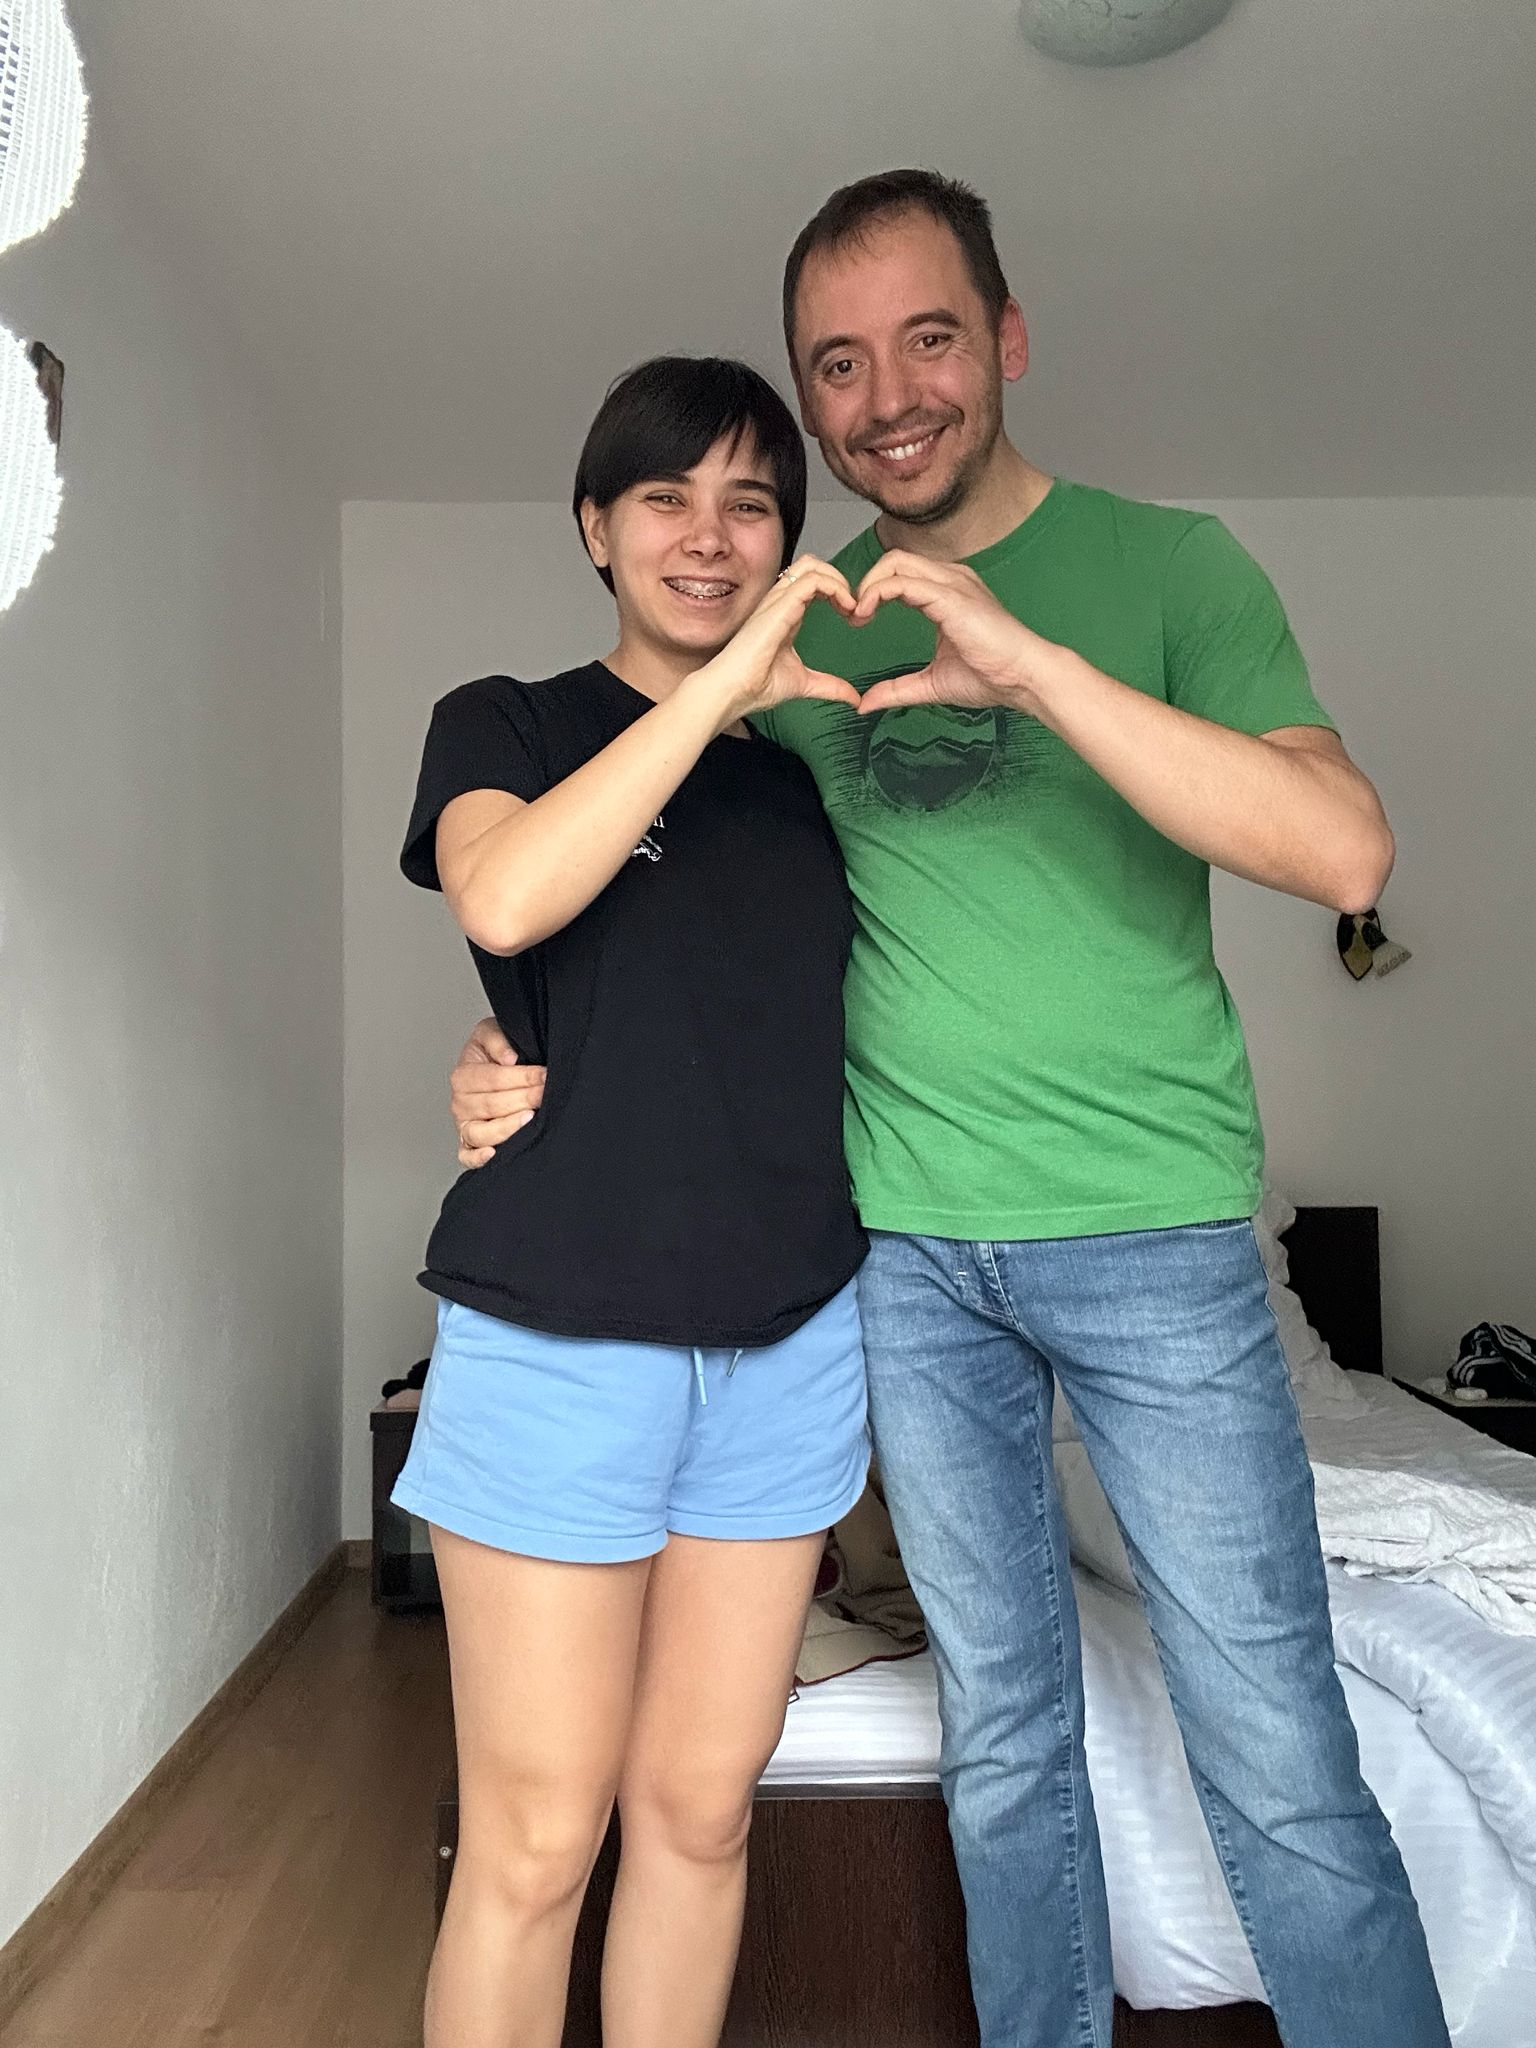
\includegraphics[width=0.45\textwidth]{img/ad-rd-heart-fingers.jpeg}
  \end{figure}
\end{frame}

\begin{frame}{La finalizare (3)}
  \centering
  \pause
  \Large
  Iubiți-vă și în felul care contează! \\
  \vspace{5mm}
  \pause
  \begin{figure}
    \centering
    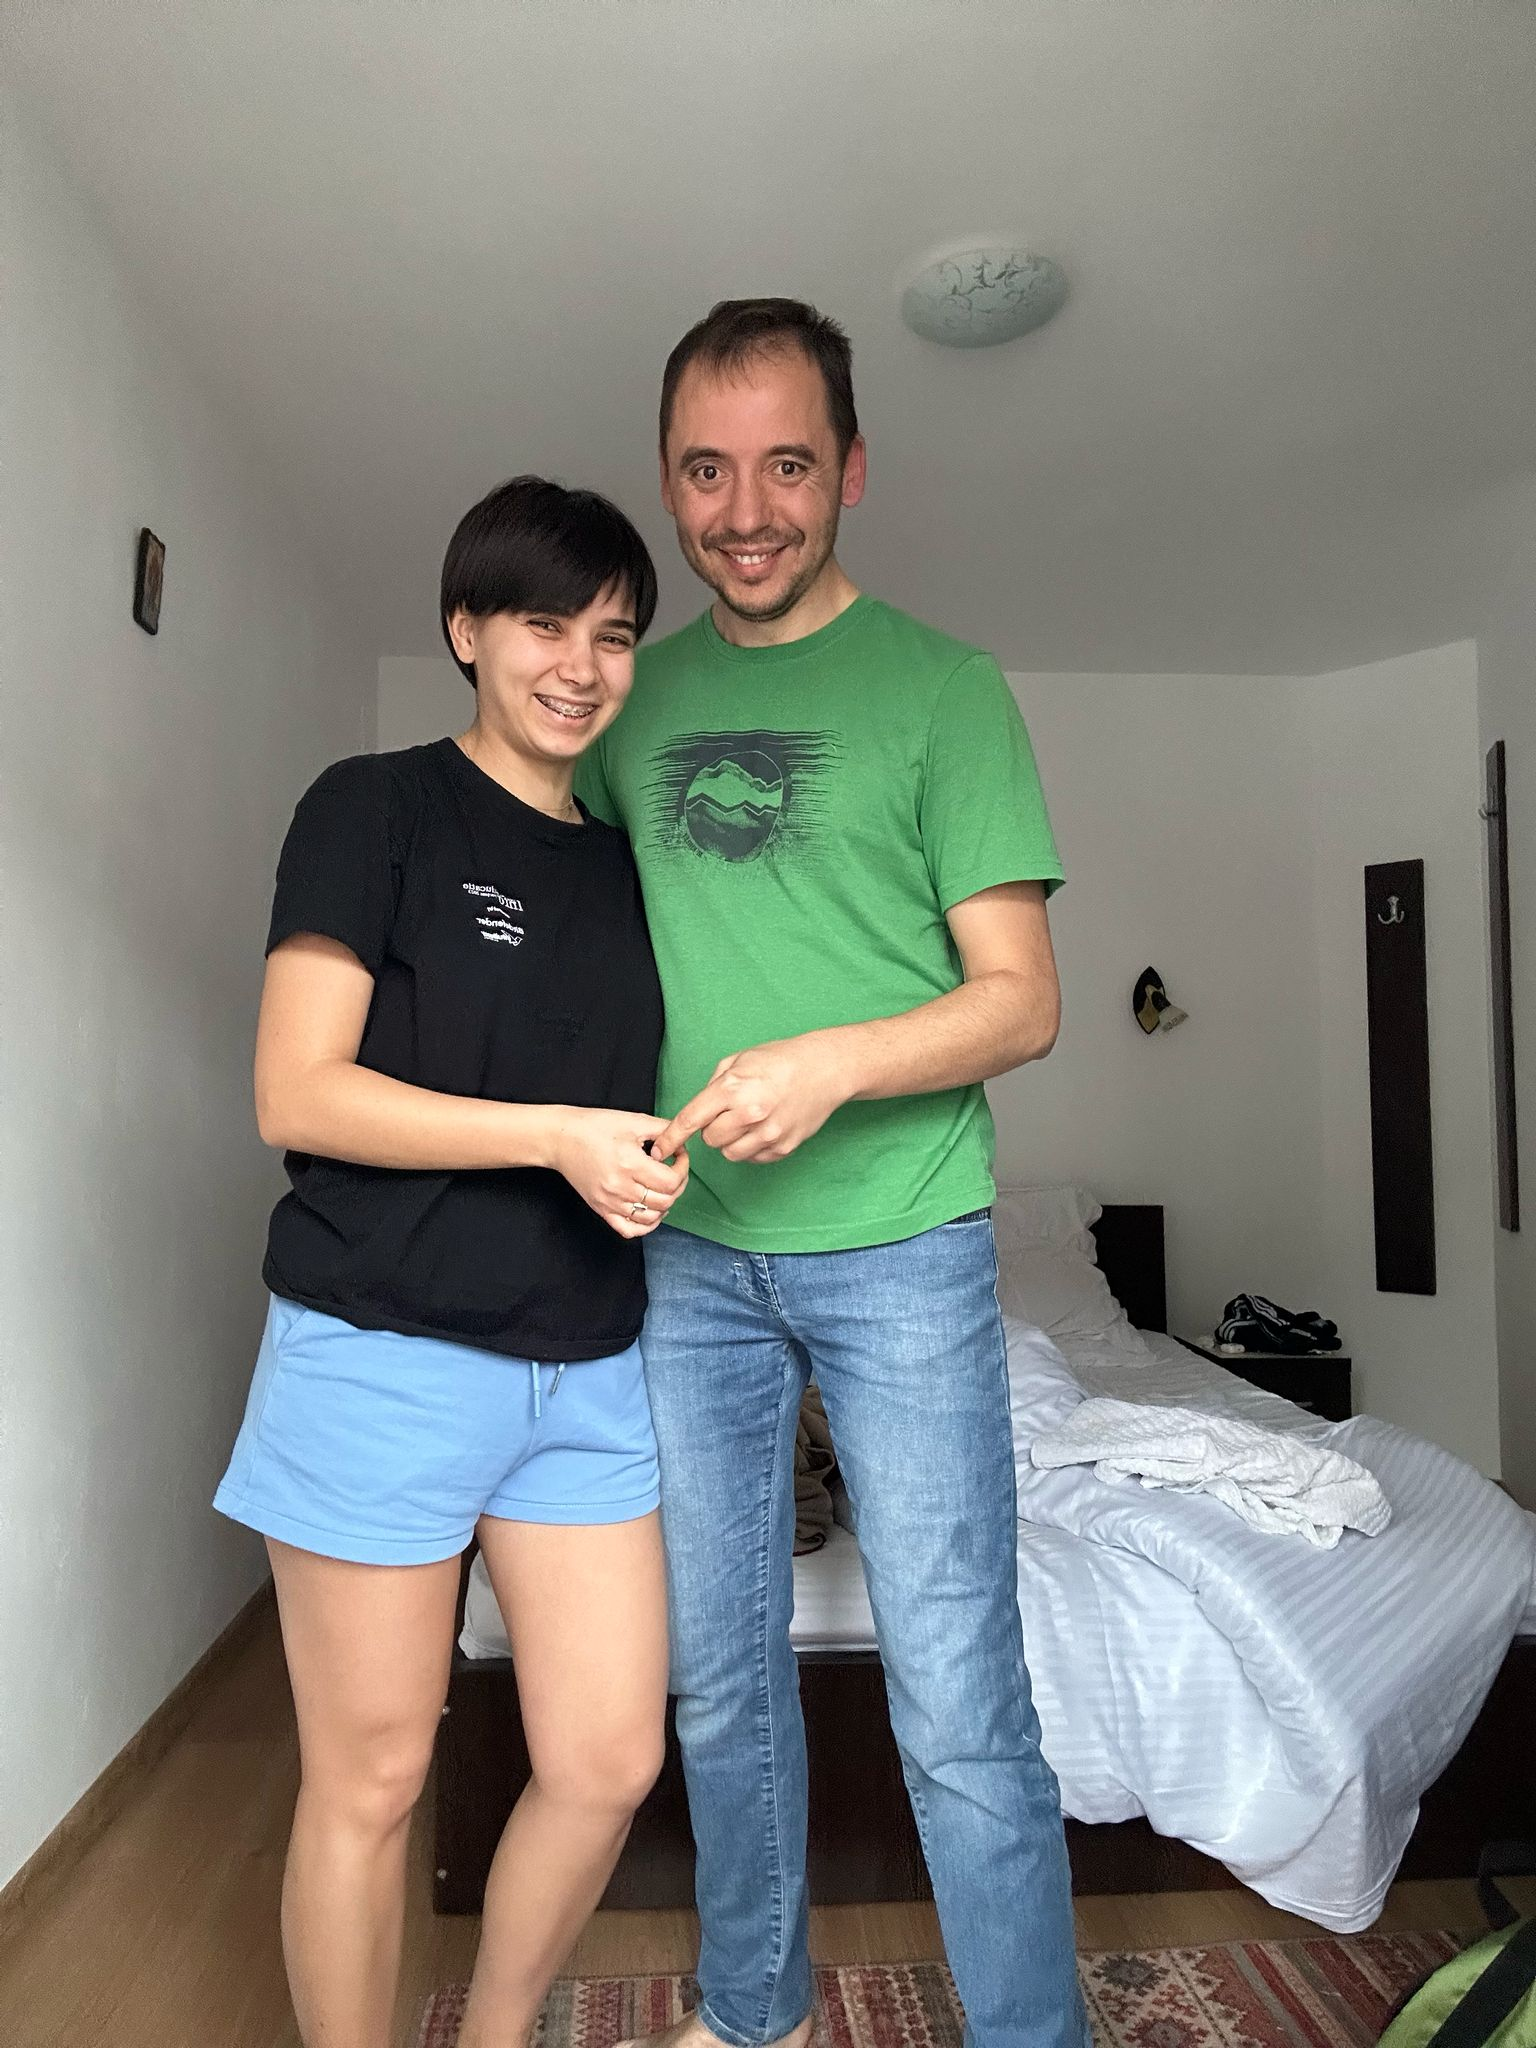
\includegraphics[width=0.45\textwidth]{img/ad-rd-finger-in.jpeg}
  \end{figure}
\end{frame}

\begin{frame}{La finalizare (4)}
  \centering
  \pause
  \Large
  Noi la bătrânețe! \\
  \vspace{5mm}
  \pause
  \begin{figure}
    \centering
    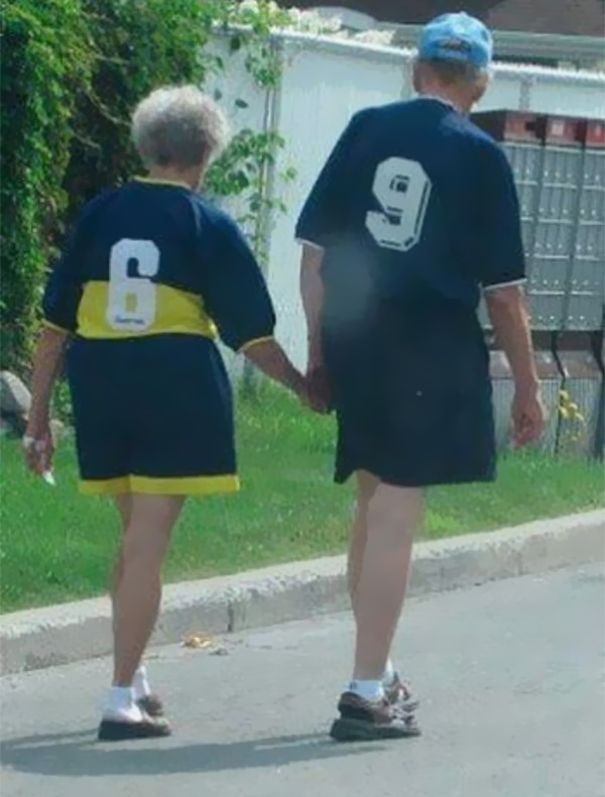
\includegraphics[width=0.45\textwidth]{img/old-couple-6-and-9.jpg}
  \end{figure}
\end{frame}

\begin{frame}{Link la slide-uri}
  \url{https://www.slideshare.net/slideshow/cum-sa-fii-bun-la-sex-dincolo-de-inhibi-ii-i-prejudeca-i/276736828}
\end{frame}

\end{document}
